\documentclass{article}
% Shared style for the LUMEN manuscript diagrams (\input by every fig_*.tex; class: article).
% Uses only fonts and packages of a basic TeX installation (Computer Modern Sans), so compiling
% never triggers a package download. Each figure is wrapped in the lumenfig environment, which
% ships the picture out as a single page cropped to the drawing plus a 3 pt margin.
\usepackage{amsmath,amssymb}
\renewcommand{\familydefault}{\sfdefault}
\usepackage{tikz}
\usetikzlibrary{positioning,arrows.meta,fit,backgrounds,calc,shapes.geometric,decorations.pathreplacing}
\pagestyle{empty}

\newsavebox{\lumenfigbox}
\newenvironment{lumenfig}%
  {\begin{lrbox}{\lumenfigbox}}%
  {\end{lrbox}%
   \pdfpagewidth=\dimexpr\wd\lumenfigbox+6pt\relax
   \pdfpageheight=\dimexpr\ht\lumenfigbox+\dp\lumenfigbox+6pt\relax
   \hoffset=-1in\voffset=-1in
   \shipout\vbox{\kern3pt\hbox{\kern3pt\usebox{\lumenfigbox}}}}

% palette: physics (blue), learning (green), data (amber), reporting (violet), neutral ink
\definecolor{ink}{HTML}{1F2933}
\definecolor{muted}{HTML}{52606D}
\definecolor{rule}{HTML}{CBD2D9}
\definecolor{phyE}{HTML}{3B6EA8}\definecolor{phyF}{HTML}{E8F1FB}
\definecolor{lrnE}{HTML}{3C8C5A}\definecolor{lrnF}{HTML}{EAF6EE}
\definecolor{datE}{HTML}{B7791F}\definecolor{datF}{HTML}{FDF3E4}
\definecolor{outE}{HTML}{6B4FA0}\definecolor{outF}{HTML}{F3EEFB}
\definecolor{grey}{HTML}{9AA5B1}

\tikzset{
  >={Stealth[length=2.4mm,width=1.8mm]},
  every node/.style={font=\footnotesize, text=ink},
  box/.style={draw, rounded corners=2.5pt, line width=0.7pt, align=center, inner sep=4pt,
    execute at begin node={\hyphenpenalty=10000\exhyphenpenalty=10000}},
  phy/.style={box, draw=phyE, fill=phyF},
  lrn/.style={box, draw=lrnE, fill=lrnF},
  dat/.style={box, draw=datE, fill=datF},
  rep/.style={box, draw=outE, fill=outF},
  neutral/.style={box, draw=grey, fill=white},
  flow/.style={->, line width=0.8pt, draw=ink},
  soft/.style={->, line width=0.7pt, draw=muted, dashed},
  title/.style={font=\footnotesize\bfseries},
  note/.style={font=\scriptsize, text=muted, align=center},
  stage/.style={draw=rule, rounded corners=4pt, line width=0.6pt, dashed, inner sep=6pt},
  stagelabel/.style={font=\scriptsize\bfseries, text=muted, anchor=south west, inner sep=1pt},
}

\begin{document}
\begin{lumenfig}
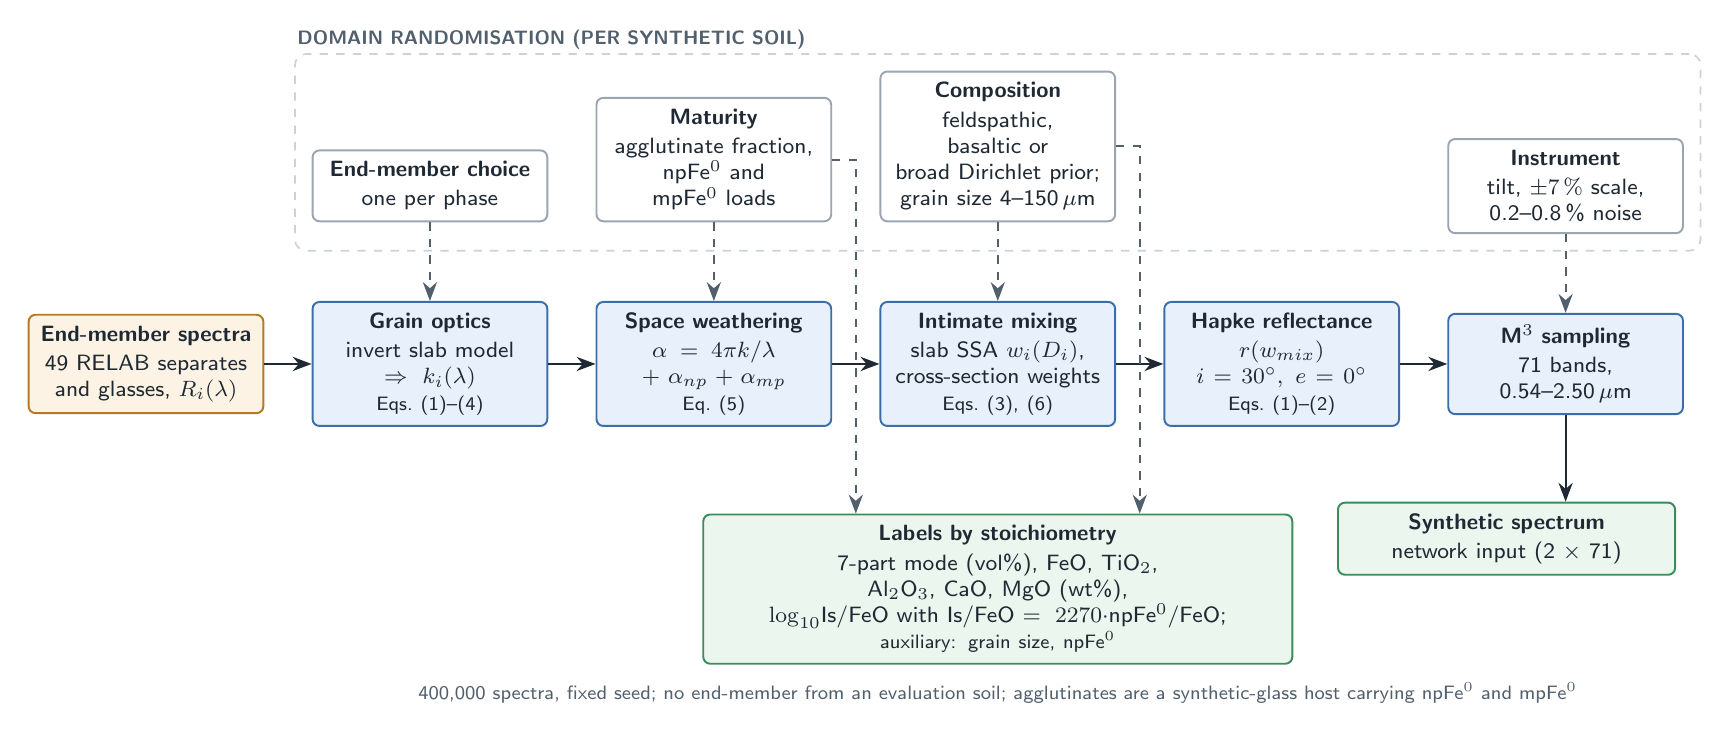
\begin{tikzpicture}[node distance=6mm and 6mm]

% ---- forward model chain (middle row)
\node[dat, text width=27mm] (em) {\textbf{End-member spectra}\\[1pt]49 RELAB separates\\and glasses, $R_i(\lambda)$};
\node[phy, text width=27mm, right=of em] (k) {\textbf{Grain optics}\\[1pt]invert slab model\\$\Rightarrow k_i(\lambda)$\\{\scriptsize Eqs.~(1)--(4)}};
\node[phy, text width=27mm, right=of k] (sw) {\textbf{Space weathering}\\[1pt]$\alpha = 4\pi k/\lambda$\\$+\ \alpha_{np} + \alpha_{mp}$\\{\scriptsize Eq.~(5)}};
\node[phy, text width=27mm, right=of sw] (mix) {\textbf{Intimate mixing}\\[1pt]slab SSA $w_i(D_i)$,\\cross-section weights\\{\scriptsize Eqs.~(3), (6)}};
\node[phy, text width=27mm, right=of mix] (hap) {\textbf{Hapke reflectance}\\[1pt]$r(w_{mix})$\\$i=30^\circ,\ e=0^\circ$\\{\scriptsize Eqs.~(1)--(2)}};
\node[phy, text width=27mm, right=of hap] (band) {\textbf{M$^3$ sampling}\\[1pt]71 bands,\\0.54--2.50\,$\mu$m};

\draw[flow] (em) -- (k);
\draw[flow] (k) -- (sw);
\draw[flow] (sw) -- (mix);
\draw[flow] (mix) -- (hap);
\draw[flow] (hap) -- (band);

% ---- random draws (top row)
\node[neutral, text width=27mm, above=10mm of k] (r1) {\textbf{End-member choice}\\[1pt]one per phase};
\node[neutral, text width=27mm, above=10mm of sw] (r2) {\textbf{Maturity}\\[1pt]agglutinate fraction,\\npFe$^0$ and mpFe$^0$ loads};
\node[neutral, text width=27mm, above=10mm of mix] (r3) {\textbf{Composition}\\[1pt]feldspathic, basaltic or\\broad Dirichlet prior;\\grain size 4--150\,$\mu$m};
\node[neutral, text width=27mm, above=10mm of band] (r5) {\textbf{Instrument}\\[1pt]tilt, $\pm7\,\%$ scale,\\0.2--0.8\,\% noise};
\draw[soft] (r1) -- (k);
\draw[soft] (r2) -- (sw);
\draw[soft] (r3) -- (mix);
\draw[soft] (r5) -- (band);
\begin{scope}[on background layer]
  \node[stage, fit=(r1)(r2)(r3)(r5)] (rnd) {};
\end{scope}
\node[stagelabel] at (rnd.north west) {DOMAIN RANDOMISATION (PER SYNTHETIC SOIL)};

% ---- outputs (bottom row)
\node[lrn, text width=40mm, below=11mm of band.south west, anchor=north west, xshift=-14mm] (spec) {\textbf{Synthetic spectrum}\\[1pt]network input (2 $\times$ 71)};
\node[lrn, text width=72mm, below=11mm of mix] (lab) {\textbf{Labels by stoichiometry}\\[1pt]7-part mode (vol\%), FeO, TiO$_2$, Al$_2$O$_3$, CaO, MgO (wt\%),\\$\log_{10}$Is/FeO with Is/FeO $= 2270\cdot$npFe$^0$/FeO;\\{\scriptsize auxiliary: grain size, npFe$^0$}};
\draw[flow] (band.south) -- (band.south |- spec.north);
\coordinate (g1) at ($(sw.east)!0.5!(mix.west)$);
\coordinate (g2) at ($(mix.east)!0.5!(hap.west)$);
\draw[soft] (r2.east) -| (g1 |- r2.south) -- (g1 |- lab.north);
\draw[soft] (r3.east) -| (g2 |- r3.south) -- (g2 |- lab.north);


\node[note, below=1mm of lab] {400{,}000 spectra, fixed seed; no end-member from an evaluation soil; agglutinates are a synthetic-glass host carrying npFe$^0$ and mpFe$^0$};
\end{tikzpicture}
\end{lumenfig}
\end{document}
